\section{Background} \label{s:background}

There are numerous game engines with their associated development environments which could be suitable for CAV development, e.g. Unreal~\footnote{\url{https://www.unrealengine.com/}}, Unity~\footnote{\url{https://unity.com/}}, CryEngine~\footnote{\url{https://www.cryengine.com/}}. Specific autonomous driving research tools have been created to abstract and simplify the development environment, some of which are based on existing engines, e.g. Carla~\footnote{\url{http://carla.org/}}, AirSim~\footnote{\url{https://microsoft.github.io/AirSim/}}, Apollo~\footnote{\url{http://apollo.auto/}}, and some have been developed for cloud based simulation, e.g. Nvidia Drive Constellation~\footnote{\url{https://www.nvidia.com/en-gb/self-driving-cars/drive-constellation/}}.

Investigating the determinism of gaming engines has not attracted much research interest since performance is more critical for playing games than accurate and repeatable runtime execution. %However, when these engines are used for CAV development then deterministic behaviour is required. 
This section gives an overview of a gaming engine and what sources or settings in the engine may affect \textit{simulation variance}.
%
% \noindent This section overviews important information and concepts in physics engines, which are relevant to their usage in CAV simulations. Particularly, on how physics engines operate and the sources of non-determinism in these engines necessary to understand the contribution of this paper.

% ======= Overview of a Game Loop
\subsection{Overview of a Game Loop} \label{GameLoopSection}
The game loop is responsible for the interaction between the physics and rendering engines. Fig.~\ref{GameEngineLoopDiagram} depicts a basic representation of the process flow in a game engine loop (initialisation, game logic and decommissioning are removed from this diagram for brevity\footnote{\url{https://docs.unity3d.com/Manual/ExecutionOrder.html}}). A game loop is broken up into three distinct phases: processing the inputs, updating the game world (Physics Engine), and generating outputs (Rendering).~\cite{GameEngineArchBook}

\begin{figure}[h]
\centering
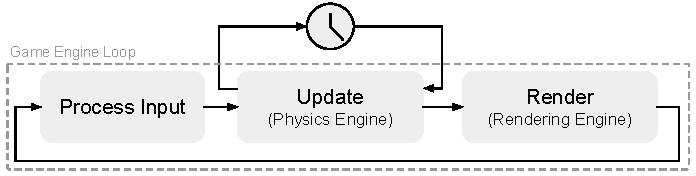
\includegraphics[width=0.5\textwidth]{Other/Figures/GameEngineLoop.pdf}
\caption{Game engine loop block diagram~\cite{GameProgPatternsBook}}
\label{GameEngineLoopDiagram}
\end{figure}
The first part of the game loop is to process the user inputs which may take the form of user keyed inputs or, in the case of CAV development, the resultant actions of the autonomous vehicle given the current state of the environment. For example, the throttle and steering inputs from the vehicle controller of an AV.
%
The update interprets the intended actions of all dynamic actors in the scene, performs any necessary physics calculations and updates the actor states. 
%
The rendering engine then takes the updated actor states and renders the scene~\cite{GameProgPatternsBook}. 
% 
% It is necessary to have an understanding of how the game loop operates in order to understand potential sources of non-determinism that are discussed below. 
% 
The key aspects of the game loop needed for this discussion are as follows: 

\begin{itemize}[leftmargin=*]
    \item At the beginning of each tick, the lag between the game clock and the real world is updated based on how much real time passed. This measures how far the game's clock is behind compared to the real world.
    \item Then the user inputs are processed.
    \item There is then an inner loop to update the physics processes (clock symbol in Fig.~\ref{GameEngineLoopDiagram}), incrementing at a delta time step, $dt$, until the game clock is equal to the real world. 
    \item Rendering occurs once the game clock has caught up with the real world clock. 
    \item The process then repeats.
\end{itemize} 

If the physics engine uses a fixed time step ($dt$), %, because it makes everything simpler and more stable for physics and AI.
the shorter this time step is the smoother the interpretation of the physical dynamics will be. %processing time it takes to catch up to game clock. % and the more deterministic the engine becomes and vice versa, as will be explained in section \ref{s:nondeterminisimSources}. 
%
To use a fixed physics time step the user's display refresh rate needs to be known in advance. This requires an update loop to take less than one render tick (one frame of real world time). Given the range of different hardware capabilities a variable delta time is often implemented for game playing taking the previous frame time as the next $dt$. However, variable $dt$ can lead to different outcomes in repeated tests and in some cases unrealistic physical representations~\cite{gaffer}. Semi-fixed or limited frame rates ensure $dt$ does not exceed some user-defined limit to meet a minimum standard of physical representation but allows computational headroom for slower hardware. Some engines provide sub-stepping which does multiple physics calculations per frame at a greater CPU cost~\footnote{\url{https://docs.unrealengine.com/en-US/Engine/Physics/Substepping/index.html}}. If the engine tries to render between updates \textit{residual lag} can occur and extrapolation between frames is performed to smooth transition between scenes, see lower part of Fig.~\ref{GameEngineLoopDiagram}. %\cite{GameEngineArchBook}\cite{GameProgPatternsBook}
%
% Ideally the time step should be as short as possible, so that the simulation returns better accuracy of complex physical processes. %runs with high fidelity on fast machines. 
In exceptional cases where resources are scarce, the fixed time step can be greater than the time between render ticks %it takes to process an ``Update" inner loop on some (slow) machines, 
and the simulation will exhibit lag between input commands and rendered states resulting in unsynchronised and unrealistic behaviour.

% The time step, $dt$, in the physics calculation is important and the smaller the value the more realistic the simulation will be. If $dt$ is too large or irregularly spaced then the rendered motion may not be smooth and interpolation may be required at additional computational cost. 

% This process allows hardware scalability, but the rendering will become of jerky quality on slower machines. These engines update at fixed intervals and render whenever they can, which is not steady. This results in what is so called residual lag\cite{GameEngineArchBook}\cite{GameProgPatternsBook}, where the engine is trying to render between two consecutive updates. In this case, the engine will use extrapolation techniques to give an estimate of where the object should be. This often is sufficient for gaming purposes and unnoticeable to the user, in fact it improves the stuttery motion.

\begin{figure*}[b]
    \centering
    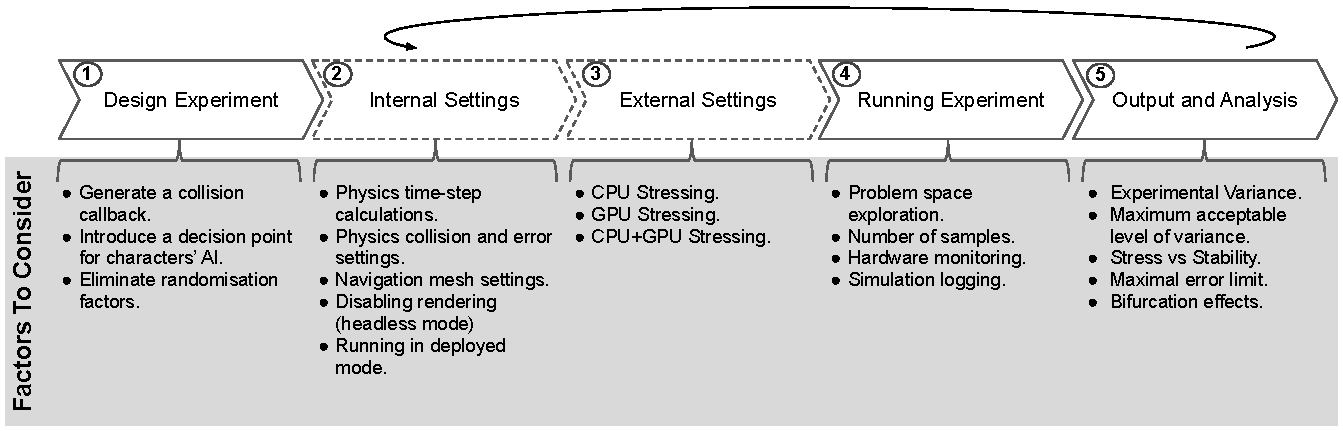
\includegraphics[width=0.99\linewidth]{Other/Figures/MethodologyDiagram.pdf}
    \caption{Shows a flow diagram of the methodology proposed to define the simulation variance of a gaming engine for usage in CAV simulations.}

    \label{method_diagram}
\end{figure*}

% ======= Sources of non-determinism
\subsection{Sources of Non-Determinism} \label{s:nondeterminisimSources}

The following points form a hypothesis around the potential sources of non-determinism that could occur in game engines. \\\\
% \noindent After establishing an understanding of how physics engines work, the focus will now be on what causes these engines to be non-deterministic. The main reasons that we think are causes of these engines' non-determinism are discussed below. \\\\

\noindent\underline{\textit{Floating Point Representation:}}
Floating point representation of real numbers is limited with fixed register sizes resulting in errors of \textit{rounding} where loss of bits occur which are rounded or truncated and \textit{cancellation} which happens where two similar values are subtracted~\cite{FloatingPointsBook,goldberg1991every}. 
%
% Translating to the usage of CAV simulations in physics engines,
This could result in precision issues of, for example, actor position within the environment and falsely satisfying or failing assertions. Such reasons would often make one jump to conclude that floating points are the cause of non-determinism, but these precision issues should be referred to as \textit{incorrectness} and not non-deterministic. Since hardware is assumed deterministic, then the same hardware should produce the same \textit{incorrect} output for the same initial conditions. So, even if the output is incorrect due to floating point precision it should always be the same, given the same logical registers which conform to the same IEEE floating point standard~\cite{8766229}. Therefore, it is unlikely that floating point representation will contribute to \textit{simulation variance} for repeated tests on the same hardware.
%
% A generic issue with computers are floating points precision. 
%Various errors occur when doing arithmetic manipulations using floating points, especially when operating between large and small numbers due to rounding, memory limitations and so forth.\cite{FloatingPointArithmeticArticle}\cite{FloatingPointsBook}. 
%Translating to the usage of CAV simulations for V\&V in physics engines, this could result in many precision issues resulting in complex non deterministic behaviours.
%
% For instance, consider a simulation where the world is infinite and progressively  generated in the physics engine. 
% After a few hundred meters, precision issues will start to occur, and will get progressively worse the further from the origin the simulation gets. 
% This is due to the values of the coordinates being used in calculations are getting bigger and hence will not cope with small values that are critical for V\&V testing purposes. 
% A solution to this problem is perhaps every time the simulations moves 100 meters away from the origin the entire world will move by 100m in the opposite direction. Thus, avoiding getting into floating point issues.\cite{FloatingPointArithmeticArticle}
%
% There are many scenarios that could be addressed, and solutions to them will entirely depend on the characteristics of that specific scenario. There is no generalised solution for the floating problem, regardless of how good computers get there will always be a limitation. However, floating points as they stand could just be sufficient for V\&V testing purposes. Whenever they are not, smart solutions can be found to accommodate for these limitations.
\\\\
\noindent\underline{\textit{Scheduling:}} %
Scheduling is a resource management method for sharing computational resources between tasks of different or competing priority where tasks are executed  dependent on the scheduler policy. A scheduler policy may be optimised in many ways such as for task throughput, deadline delivery or minimum latency~\cite{liu1973scheduling}. 
%
If during simulation the scheduling policy was updated or thread priority was inconsistently handled then variance in output may be expected. It is, however, unlikely that such events would occur on repeated controlled tests for the same hardware and operating system configuration. %
%
Similar to thread scheduling, the CPU scheduling policy determines which processor core to execute processes in the ready queue and this is maybe ordered by factors such as throughput, latency and CPU utilisation. %
%
If the same single-threaded script executes multiple times across different physical cores due to the CPU utilisation policy then should this be considered deterministic? Processor designs should be identical although impurity inconsistency across the bulk silicon and minor perturbations in the semiconductor processing across the chip may exist. End users expect such minor variations to be controlled for in architecture design and factory testing.

Another issue to consider is concurrency, where sequential tasks can be executed out of order to improve speed by utilising parallelisation although it depends on the decomposability of the program. This technique can lead to issues such as shared resource access conflicts and RACE conditions~\cite{huffman1954synthesis}. 


Scheduling of threads may be a reason for non-deterministic simulation behaviour in game engines. Given the same hardware the output should always be the same, unless scheduling of the threads change. 
% i.e. the utilisation of hardware is manipulated differently each time. This would then result in non-deterministic behaviours especially if it is combined with the floating point problem discussed earlier. 
%
% For example, if a process on thread 1 requires data from thread 2, but thread 2 is delayed due to additional load then synchrony between the threads may be lost if not controlled for explicitly. Given that game engines will promote performance over accuracy the process on thread 1 may be dropped or skipped until the data are available. This may lead to events happening out of order depending on the computational load and hence non-deterministic.
%
% To solve the scheduling of threads problem, one would have to control all of the threads during runtime, which is very involved. To achieve that one would need to replace or control the whole run-time system to allocate tasks to the same threads in the same order. This is beyond the scope of our work and will not be covered in this paper.
\\\\
\noindent\underline{\textit{Physics and Rendering clocks:}}
% The inherent way of how these physics engines operate (i.e.game loops) causes the engine to be non-deterministic.  A follow up from section \ref{GameLoopSection}, these
Some game engines use a variable frame rate, which is good for hardware scalability but creates a challenge for the physics engine which works best with small fixed time steps. %
%
The problem of having a variable frame rate could also contribute to the non-deterministic behaviour of these engines, especially combined with loss of thread scheduling synchrony. 
%
That is to say, if the frame rate is allowed to vary then it has to be controlled to give the same variability through out a given test in order for the test results to be repeatable. This issue might be of negligible significance if the frame rate is consistent and the time steps are small enough. 
\\\\
\noindent\underline{\textit{Actor Navigation:}}
Game engines often use navigation meshes for actor path planning, which should be considered as a potential source of non-deterministic behaviour, e.g.%. Some CAV simulator developers claim that the built-in physics engines' AI is non-deterministic
~\cite{CARLABenchmark}. 
This may depend on the algorithms used by the engine which typically use the A* algorithm\cite{AStarBook} and should give deterministic outcomes as long as the environment is deterministic\cite{AirsimUnrealArticle}\cite{UnrealAIDocumentation}. 
Therefore, the determinism of the actor path planning depends on the environment and the update to actor states within it and how navigation meshes are created or modelled, e.g. shape, granularity. 
%
It is interesting to note that changes can occur to navigation meshes if they are dynamically loaded as the simulation proceeds which can reduce computational load for large area maps~\footnote{\url{https://docs.unrealengine.com/en-US/BlueprintAPI/AI/Navigation/RegisterNavigationInvoker/index.html}}. %This non-deterministic behaviour can be also resorted to the different scheduling of threads, hence giving variations in meshes every time they are loaded.


